\documentclass[a4paper,11pt]{book}
%\documentclass[a4paper,twoside,11pt,titlepage]{book}
\usepackage{listings}
\usepackage[utf8]{inputenc}
\usepackage[spanish]{babel}

% \usepackage[style=list, number=none]{glossary} %
%\usepackage{titlesec}
%\usepackage{pailatino}

%\decimalpoint
\usepackage{dcolumn}
\usepackage{float}
\newcolumntype{.}{D{.}{\esperiod}{-1}}
\makeatletter
%\addto\shorthandsspanish{\let\esperiod\es@period@code}
\makeatother


%\usepackage[chapter]{algorithm}
\RequirePackage{verbatim}
%\RequirePackage[Glenn]{fncychap}
\usepackage{fancyhdr}
\usepackage{graphicx}
\usepackage{afterpage}

\usepackage{longtable}

\usepackage[pdfborder={000}]{hyperref} %referencia

% ********************************************************************
% Re-usable information
% ********************************************************************
\newcommand{\myTitle}{Trabajo Investigación SOA\xspace}
\newcommand{\myDegree}{MÁSTER EN INVESTIGACIÓN EN INGENIERÍA DE SOFTWARE Y
SISTEMAS INFORMÁTICOS\xspace}
\newcommand{\myName}{César Hugo Bárzano Cruz\xspace}
\newcommand{\myProf}{Nombre Apllido1 Apellido2 (tutor1)\xspace}
\newcommand{\myOtherProf}{Nombre Apllido1 Apellido2 (tutor2)\xspace}
%\newcommand{\mySupervisor}{Put name here\xspace}
\newcommand{\myFaculty}{ Universidad Nacional de Educación a Distancia\xspace}
\newcommand{\myFacultyShort}{UNED-Facultad de informática\xspace}
\newcommand{\myDepartment}{\xspace}
\newcommand{\myUni}{\protect{ Universidad Nacional de Educación a Distancia}\xspace}
\newcommand{\myLocation}{Madrid\xspace}
\newcommand{\myTime}{\today\xspace}
\newcommand{\myVersion}{Version 0.1\xspace}


\hypersetup{
pdfauthor = {\myName hugobarzano@gmail.com},
pdftitle = {\myTitle},
pdfsubject = {},
pdfkeywords = {},
pdfcreator = {LaTeX con el paquete TEXmaker},
pdfproducer = {pdflatex}
}

%\hyphenation{}


%\usepackage{doxygen/doxygen}
%\usepackage{pdfpages}
\usepackage{url}
\usepackage{colortbl,longtable}
\usepackage[stable]{footmisc}
%\usepackage{index}

%\makeindex
%\usepackage[style=long, cols=2,border=plain,toc=true,number=none]{glossary}
% \makeglossary

% Definición de comandos que me son tiles:
%\renewcommand{\indexname}{Índice alfabético}
%\renewcommand{\glossaryname}{Glosario}

\pagestyle{fancy}
\fancyhf{}
\fancyhead[LO]{\leftmark}
\fancyhead[RE]{\rightmark}
\fancyhead[RO,LE]{\textbf{\thepage}}
\renewcommand{\chaptermark}[1]{\markboth{\textbf{#1}}{}}
\renewcommand{\sectionmark}[1]{\markright{\textbf{\thesection. #1}}}

\setlength{\headheight}{1.5\headheight}

\newcommand{\HRule}{\rule{\linewidth}{0.5mm}}
%Definimos los tipos teorema, ejemplo y definición podremos usar estos tipos
%simplemente poniendo \begin{teorema} \end{teorema} ...
\newtheorem{teorema}{Teorema}[chapter]
\newtheorem{ejemplo}{Ejemplo}[chapter]
\newtheorem{definicion}{Definición}[chapter]

\definecolor{gray97}{gray}{.97}
\definecolor{gray75}{gray}{.75}
\definecolor{gray45}{gray}{.45}
\definecolor{gray30}{gray}{.94}

\lstset{ frame=Ltb,
     framerule=0.5pt,
     aboveskip=0.5cm,
     framextopmargin=3pt,
     framexbottommargin=3pt,
     framexleftmargin=0.1cm,
     framesep=0pt,
     rulesep=.4pt,
     backgroundcolor=\color{gray97},
     rulesepcolor=\color{black},
     %
     stringstyle=\ttfamily,
     showstringspaces = false,
     basicstyle=\scriptsize\ttfamily,
     commentstyle=\color{gray45},
     keywordstyle=\bfseries,
     %
     numbers=left,
     numbersep=6pt,
     numberstyle=\tiny,
     numberfirstline = false,
     breaklines=true,
   }

% minimizar fragmentado de listados
\lstnewenvironment{listing}[1][]
   {\lstset{#1}\pagebreak[0]}{\pagebreak[0]}

\lstdefinestyle{CodigoC}
   {
	basicstyle=\scriptsize,
	frame=single,
	language=C,
	numbers=left
   }
\lstdefinestyle{CodigoC++}
   {
	basicstyle=\small,
	frame=single,
	backgroundcolor=\color{gray30},
	language=C++,
	numbers=left
   }


\lstdefinestyle{Consola}
   {basicstyle=\scriptsize\bf\ttfamily,
    backgroundcolor=\color{gray30},
    frame=single,
    numbers=none
   }


\newcommand{\bigrule}{\titlerule[0.5mm]}


%Para conseguir que en las páginas en blanco no ponga cabecerass
\makeatletter
\def\clearpage{%
  \ifvmode
    \ifnum \@dbltopnum =\m@ne
      \ifdim \pagetotal <\topskip
        \hbox{}
      \fi
    \fi
  \fi
  \newpage
  \thispagestyle{empty}
  \write\m@ne{}
  \vbox{}
  \penalty -\@Mi
}
\makeatother

\usepackage{pdfpages}
\begin{document}
\begin{titlepage}
 
 
\newlength{\centeroffset}
\setlength{\centeroffset}{-0.5\oddsidemargin}
\addtolength{\centeroffset}{0.5\evensidemargin}
\thispagestyle{empty}

\noindent\hspace*{\centeroffset}\begin{minipage}{\textwidth}

\centering

\includegraphics[width=0.7\textwidth]{imagenes/Logo-uned.jpg}\\[1.1cm]


{\Huge\bfseries Máster Universitario En Investigación En Ingeniería De Software Y Sistemas Informáticos\\
}
\noindent\rule[-1ex]{\textwidth}{3pt}\\[3.5ex]
{\large\bfseries Generación Automática de Código}
\end{minipage}

\vspace{2.5cm}
\noindent\hspace*{\centeroffset}\begin{minipage}{\textwidth}
\centering

\textbf{Autor}\\ {César Hugo Bárzano Cruz}\\[2.5ex]


\includegraphics[width=0.3\textwidth]{imagenes/Logo-master.png}\\[0.1cm]
\textsc{Trabajo 1 De Evaluación Continua}\\
\textsc{---}\\
2017/2018
\end{minipage}
%\addtolength{\textwidth}{\centeroffset}
%\vspace{\stretch{2}}
\end{titlepage}




%\frontmatter
\tableofcontents
\listoffigures
%\listoftables

%
%\mainmatter
%\setlength{\parskip}{5pt}

%\input{capitulos/01_Introduccion}


\chapter{Introducción}

El presente documento representa la memoria formal para el trabajo de investigación de la asignatura Arquitecturas Orientadas a Servicios. Dicho trabajo consta de 2 bloques principales.


En la primero de ellos, se daran ejemplos de arquitecturas orientadas a servicios en un contexto laboral y empresarial, haciendo distintcion entre soluciones exitosas y soluciones no tan funcionales. En el segundo, se abordará de una manera más práctica el análisis, diseño e implementación de una arquitectura orientada a servicios con el objetivo de solucionar un problema planteado con este tipo de arquitecturas así como las tecnologías relacionadas con ellas. 

\chapter{Soluciones SOA}

En la actualidad, las tecnolgías web así como las soluciones basadas en servicios cloud han tomado un gran peso tanto en nuestra vida cotidíana como para el mundo empresarial. El paradigma de servicios cloud denominado "La WEB 2.0" ha revolucionado la manera en la que la información llega al usuario.  El valor aportado al mundo empresarial por el tratamiendo de datos para la toma de decisiones junto con la trasnformación digital ha hecho que innumerables empresas se suban al carro de las nuevas tecnologías ya que una pequeña inversión en innovación marca una notable mejora en sus procesos de negocio.

Cada vez son más las soluciones basadas en arquitecturas orientadas a servicios que el usuario tiene a su disposición y cada vez son más diversas las necesidades tecnológicas y servicios de la información que tanto ususarios como empresas requiere. Por ello, en los ultimos años, han surgido ciertos proveedores de servicios con soluciones basadas en SOA que se han convertido en el buque insignia de las tecnologías cloud. Los proveedores de soluciones SOA para "La WEB 2.0" que se tratarán a continuación son:  

\begin{enumerate}
\item \textbf{Google Cloud Platform}
\item \textbf{Amazon Web Services}
\item \textbf{Microsoft Azure}
\item \textbf{Mlab}
\item \textbf{Yahoo!}
\end{enumerate}

De manera adicional se comentará brevemente Ether Cloud Services, la plataforma cloud hibrida con base de gobierno presentada por el banco BBVA para este 2018 en el evento Ether.io de noviembre, plataforma en la que actualmente desempeño el rol de desarrollador de soluciones. 

\subsection{Google Cloud}

Google Cloud\cite{google}, es una plataforma en la nube que ha unificado las aplicaciones para el desarrollo de aplicaciones cloud ofrecidas por Google. Permite crear soluciones  eficientes y escalables. Ejemplos de aplicaciones basadas en SOA pueden ser las propias ofertadas por Google ya que estan basadas en su infraestructura cloud: 

\begin{enumerate}
\item \textbf{Gmail}
\item \textbf{Google Drive}
\item \textbf{Google Sites}
\item \textbf{Google Contacts}
\item \textbf{Google Apps para educación}
\end{enumerate}

Aunque Google pone a disposición de los usuarios bastantes aplicaciones o servicios de caracter gratuito, el principal problema para los desarrolladores de arquitecturas basadas en microservicios es la facturación. Esta puede ser por unidades de cómputo o almacenamiento por lo que un correcto analisis y diseño de la infraestructura virtual que va a soportar la arquitectura basada en servicios que el desarrollador o desarrolladores han de implementar, asi como un análisis del tráfico o concurrencia que dicha SOA ha de soportar puede suponer una correcta decisión o no el usar los servicios cloud ofertados por Google. 

Se considera una SOA exitosa debido al número de usuarios activos que dicha plataforma tiene en todo el mundo, así como la adecuada experiencia de usuario que ofrece. 

\subsection{Amazon Web Services}

AWS\cite{aws} es una colección de servicios cloud ofrecidos por Amazon bajo el abanico de su nube pública.  (también llamados servicios web) que en conjunto forman una plataforma de computación en la nube, ofrecida a través de Internet. Algunos ejemplos exitosos de aplicaciones basadas en SOA que a su vez hacen uso de una arquitectura orientada a servicios como ofrece la plataforma de Amazon son:

\begin{enumerate}
\item \textbf{Dropbox}
\item \textbf{Foursquaree}
\item \textbf{HootSuite}
\end{enumerate}

La principal ventaja y a la vez problema de la nube de Amazon es su categorización de servicio por regiones o zonas de disponibilidad que se indican en la tabla de abajo. La división de sus usuarios en las requiones que por localización geográfica mejor servicio ofrezca produce una experiencia de usuario realmente buena, equilibrando el trafico de su infraestructura cloud pero debido a las distintas legislaciones en cuanto a la protección de datos, hay ciertas regiones en las que el almacenamiento masivo de datos de caracter sensible conlleva ciertas responsabilidades. Por ejemplo un desarrollador financiero no siempre podrá alojar sus servicios en l región de disponibilidad que el considere mejor para la latencia del mismo, si no que le vendrá impuesta por contrato o proyecto. 

Se considera un ejemplo de arquitectura basada en servicios muy exitosa debido al gran número de usuario que tiene en todo el mundo. De manera adicional, AWS facilita el aprendizaje de su tecnología a estudiantes proporcionando horas de cómputo y unidades de almacenamiento a los propietarios de cuentas de correo universitario. 

\begin{figure}[H]  
\centering 
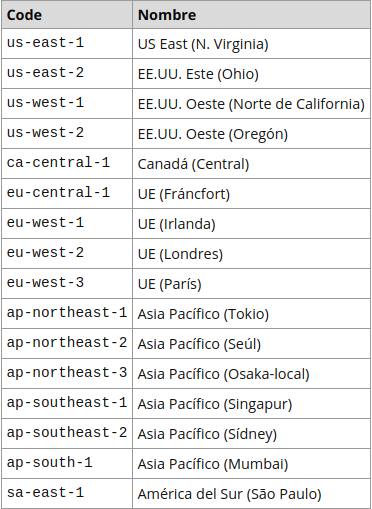
\includegraphics[scale=0.35]{imagenes/zonas.png}
\caption{ Regiones de Diponibilidad }  
\end{figure} 

\subsection{Microsoft Azure}

Microsoft Azure\cite{azure} es conjunto de servicios cloud de caracter empresarial para solucines comerciales. Azure cuenta con un amplio abanico de servicios, herramientas y frameworks para la creación y administracion de soluciones web a nivel mundial. Se le considera un triunfador en el mundo se los servicios cloud, con su gigantesca arquitectura basada en servicios se presenta como un pionero en el mundo de las soluciones cloud. A pesar de que Azure facilita el aprendizaje de su tecnología a los estudiantes concediendo paquetes de computo se la considera una de las plataformas cloud mas caras en terminos de computo y almacenamiento. 

\subsection{mLab}

mLab\cite{mlab} se caracteriza por ser un servicio de base de datos cloud que ofrece capacidad de almacenamiento en forma de base de datos relacional, MongoDB. mLab proporviona a sus usuarios un servicio de base de datos no relacional totalmente administrado que se ejecuta sobre proveedores de servicio como los vistos anteriormente (Google, Amazon o Microsoft Azure)

Se considera un ejemplo de SOA exitoso debido a que el servicio ofertado es consumido por miles de desarrolladores cloud en todo el mundo para implementar soluciones SOA ademas de facilitar el aprendizaje de su tecnología de negocio ya que ofrece pequeñas parcelas de almacenamiento cloud de manera gratuita. 

\subsection{Yahoo!}

Yahoo\cite{yahoo} es un portal de internet que ofrece distintos servicios de información como correo electrónico, directorio de servicios web y principalmente motor de busqueda. La arquitectura de este portal esta basada en el paradigma de las arquitecturas basadas en microservicios pero es considera como un fracaso empresarial ya que en En 2009, Yahoo anunció que en el primer trimestre sus utilidades cayeron 78\% con respecto a igual periodo de 2008. La compañía despidió a más de 5\% de su personal, equivalente 700 empleados, que se sumaban a 
los 1500 anunciados el mismo año. La compañía no podía hacer frente a Google, su principal rival por lo que en 2012 despidío a 2000 empleados, el 14\% de su equipo global. 

\subsection{Ether Cloud Services}

ECS\cite{ecs} se presenta como el futuro competidor de AWS y Google Cloud para desarrolladores de servicios y soluciones financieras sobre escenarios cloud. La plataforma ECS presenta un conjunto de diversas disciplinas de servicios cloud con base de gobierno para el desarrollo y despliegue de aplicaciones basadas en servicios. La plataforma en si es una arquitectura SOA pura en la que un conjunto de piezas o servicios, implementando unas interfaces o End-points comunes son capaces de formar una red cloud a nivel global para ofrecer todo tipo de servicios para desarrolladores de aplicaciones financieras, análisis continuo de flujos de datos, categorización, aprovisionamiento, testing, cómputo y almacenamiento en todo el mundo, permitiendo asi que los procesos de negocio del banco cambien de modo BATCH a REAL-TIME.  

\chapter{Aplicación Técnica SOA}

Como segunda parte del trabajo de investigación se va a realizar la especificación, análisis e implementación de un sistema cuya arquitectura esta basada en servicios. 

\section{El Problema}

Como desarrolladores de soluciones, cliente ha solicitado un sistema para el tratamiento y procesamiento de datos. Cliente indica que el producto ha de ser capaz de manejar distintos conjuntos de datos muy variados. De manera adicional, el producto resultante ha de ser capaz de realizar ciertas operaciones sobre los conjuntos de datos. Una de las principales preocupaciones del cliente es su escalabilidad ya que en etapas tempranas del proyecto, el sistema no tendrá mucho tráfico pero en versiones futuras, el número de usuarios a los que tendrá que dar servicio podría expresarse en terminos globales, por lo que el sistema ha de ser rápido, eficiente y facilmente escalable.

\section{Análisis del Problema}

Para abordar el problema planteado por cliente, se ha decidido utilizar una arquitectura basada en microservicios. Para ello, se pretende definir un bloque principal para la gestión de los conjuntos de datos o datasets. Cliente será capaz de interaccionar con el bloque de gestión mediante una API-RESTFUL\cite{api} basada en protocolo HTTP\cite{http}, lo que le permitirá consumir el servicio de datos y usar el sistema como back-end para implementar aplicaciones que consuman dicho servicio de tratamiento de datos de una manera sencilla y homogenea. De manera adicional y usando dicha interfaz REST, el cliente será capaz de realizar operaciones sobre los conjuntos de datos que  el sistema es capaz de gestionar. Con el objetivo de optimizar el rendimiento y la eficiencia se ha decidido delegar el procesamiento de datos a otro servicio totalmente independiente al bloque principal de gestión, por lo que tanto el bloque de gestión como los servicios esclavos encargados del tratamiento de datos, deberan implementar una API-REST privada. De esta forma, la experiencia que percibe el usuario será trasnparente al procesamiento que el sistema realice en su interior, ya que cliente solo conocerá la API publica del bloque de gestión. 

Este paradigma permitirá al sistema escalar fácilmente e incluir nuevas operaciones o tratamientos para los datos que el bloque de gestión disponibiliza mediante la API pública a cliente. El siguiente diagrama muestra la arquitectura basada en servicios rest que se quiere desarrollar para solucionar el problema propuesto. 


\begin{figure}[H]  
\centering 
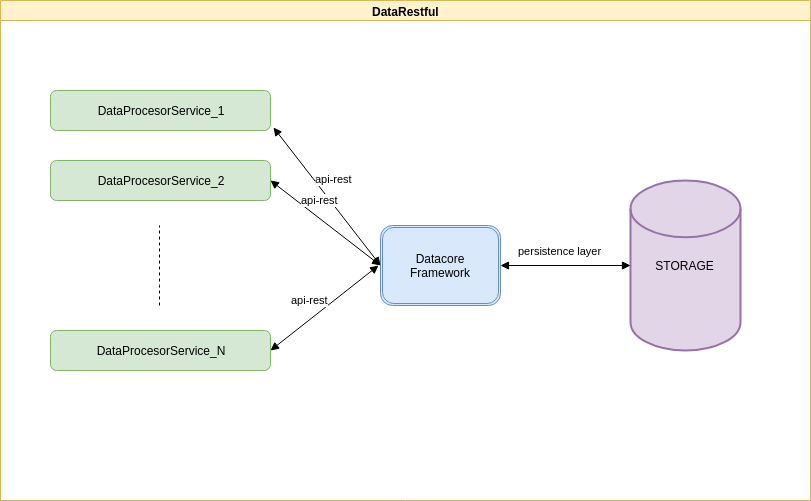
\includegraphics[scale=0.35]{imagenes/arquitectura_datarest.png}
\caption{ Arquitectura SOA }  
\end{figure} 

Podemos distinguir 3 elementos o conceptos principales dentro del sistema propuesto, bautizado como Datarestful:

\begin{enumerate}
\item \textbf{Procesadores}
\item \textbf{Datacore}
\item \textbf{Almacenamiento}
\end{enumerate}


Para el usuario y su experiencia con el sistema, esto es transparente pues el realizará peticiones a Datarestful nivel sistema mediante la Api pública expuesta por el Datacore o framework a nivel sub-sistema y delegadas al resto del subsistemas dependiendo de si se requiere cómputo, almacenamiento o ambos mediante la Api privada no accesible para ususarios, si no solo para los servicios que formen parte de la aquitectura SOA que forma Datarestful. 

\subsection{Procesadores}

Encargados del procesamiento y tratamiendo de datos, son los encargados del procesamiento y tratamiento de datos, ofrecen servicio al core del sistema mediante Api-Rest privada. Su objetivo es la computación por lo que carecen de capa de persistencia, reciben conjuntos de datos y devuelven el resultado de aplicar cierta operación sobre ese conjunto de datos. 

\subsection{Datacore}

Framework encargado de gestionar los conjuntos de datos, su tarea es la de proporcionar al usuario una interfaz rest para manejar los datos y solicitar operaciones sobre los mismos. Carece de capacidad computacional pues todas las operaciones son delegadas a los servicios de procesamiento registrados en él. Datacore es el encargado de interactuar con la capa de persistencia implementando las operaciones CRUD necesarias para interactuar con la base de datos.  

\subsection{Storage}

Capa de persistencia encargada del almacenamiento de datos.  

\section{Especificación de la Solución}

Tras analizar el problema a resolver, en esta sección se realizará la espeficación necesaria para su solución. Para ello, se van a definir los siguientes sub-secciones: 

\subsection{Requisitos de Información del Sistema}

Los requisitos de información se caracterizan por reunir la información relevante para el cliente, es decir, que debe gestionar y almacenar el sistema software.\\

\textbf{RI-1. Dataset:} Representación de cada uno de los conjuntos de datos en el sistema. 
Contenido: ID unico del conjunto de datos, título representativo del dataset, fecha de creación y el conjunto de datos en si. \\


\textbf{RI-2. Operación:} Representación de cada una de las operaciones computacionales que el sistema pone a disposición del ususario. Contenido: ID único de la operacion, operador o palabra reservada para realizar la operación, datasets que estan involucrados en la operación. \\

\textbf{RI-3. Servicio:} Representación de cada uno de los servicios operacionales registrados en el sistema, capaces de realizar operaciones sobre conjuntos de datos. Contenido: ID único del servicio, Título del servicio, url mediante la cual se ofrece el servicio. \\

\subsection{Requisitos Funcionales del Sistema}

Como se define en la ingeniería de requisitos, los requisitos funcionales establecen los comportamientos del sistema.\\ 

\textbf{RF-1. Gestión de datasets:} El sistema será capaz gestionar el ciclo de vida de los datasets existentes en el sistema.\\
   

	RF-1.1. El sistema permitirá añadir datasets.

	RF-1.2. El sistema permitirá buscar datasets.

	RF-1.3. El sistema permitirá modificar datasets.

	RF-1.4. El sistema permitirá eliminar datasets.


\textbf{RF-2. Tratamiento de Datos:} El sistema deberá disponibilizar al usuario una serie de operaciones sobre los conjuntos de datos. \\   


	RF-2.1. El sistema permitirá realizar una operacion sobre uno o mas conjuntos de datos. 

	RF-2.2. El sistema permitirá consultar las operaciones disponibles. 

	RF-2.3. El sistema permitirá crear nuevos conjuntos de datos mediante el resultado de una o más operaciones. 

	RF-2.4. El sistema permitirá programar operaciones para ser realizadas en determinados momentos del día. 
	
\subsection{Requisitos No Funcionales del Sistema}

Los requisitos no funcionales, se refieren a todos los requisitos que no describen información a guardar, ni funciones a realizar por el sistema, sino características de funcionamiento.\\


\textbf{RNF-1} Necesitaremos que toda la información que se almacena sobre el sistema se mantenga segura, realizando copias de seguridad periódicas. \\

\textbf{RNF-2} Necesitaremos que los conjuntos de datos esten disponibles de manera rápida. \\

\textbf{RNF-3} Necesitaremos disponer de una buena conexión a internet ya que el sistema da servicio desde la nube. \\ 


\section{Implementación y Tecnológia}

Una vez realizado el análisis del problema y especificada la posible solución es el momento de tomar las decisiones adecuadas para la correcta implementación de Datarestful. De manera general, los servicios que forman el sistema han de implementar ciertos End-points o interfaces de comunicación que les permita interactuar entre ellos y con el ususario, para ello, se hará uso de HTTP (Hypertext Transfer Protocol) es un protocolo de comunicación que permite las transferencias de información en la web. 

Como se vió en el apartado "Análisis del Problema" hay 3 bloques principales que trataremos a continuación:  

\subsection{Procesadores}

Para la implementación de un procesador basíco al que el sistema pueda solicitar operaciones sobre los datasets, se ha decidido utilizar Python\cite{py}, mediante el micro-framework Flask\cite{flask} para el desarrollo de aplicaciónes web. Se ha decidido utilizar python como tecnoloǵia base debido a la gran variadad de librerias y algoritmos para el tratamiento de datos que existen para este lenguaje, muchas de ellas son adaptaciones de librerias pertenecientes al popular lenguaje para mineria de datos denominado R. 

La ventaja de la aquitectura basada en servicios que se va a implementar reside en que la tecnología utilizada es independiente al problema, es decir, el sistema puede delegar las operaciones computacionales a distintos servicios de procesado y estos pueden estar implementados con diversas tecnológias como python, javascript, scala...lo unico que han de hacer es implementar los End-points o interfaces rest que se definan en el API privada para que el sistema pueda delegar tareas computacionales a dichos servicios.

\subsection{Datacore}

Como se especificó anteriormente, Datacore es la pieza encargada de orquestar las peticiones de los usuarios con los servicios de cómputo y almacenamiento por eso se ha decidido impementar utilizando el lenguaje de programación GO\cite{go}. Esta tecnología esta orientada al desarrollo de servicios rest de altas prestaciones, optimizando el trafico y las peticiones concurrentes. Al tratarse de un lenguaje compilado, los ejecutables generados son multiplataforma lo que facilita su despliegue sobre diversas infraestructuras. 

\subsection{Store}

Como capa de persistencia se ha decidido utilizar un modelo NO relaccional, lo que permite almacenar datasets como documentos, esto significa que el enrriquecimiento de las estructuras de datos almacenadas puede realizarse de manera simple. Para ello, se ha decidido utilizar el motor NoSql proporcionado por MongoDB\cite{mongo}. Este software permite optimizar las busquedas de datasets mediante la indexación de sus colecciones de documentos lo que supone una ganacia en eficiencia con respecto a bases de datos relaccionales orientadas a transaciones de objetos como Postgresql o Mysql.   

\subsection{Virtualización}

Con el objetivo de facilitar el uso y la distribución de Datarestful como proyecto software se ha decidido utilizar el motor de virtualización ligera docker\cite{docker} para ejecutar las piezas (datacore, procesador y store) a nivel subsistema sin necesidad de obligar al desarrollador a instalarse las dependencias necesarias o a tener un servicio de sistema de gestión de bases de datos no relaccionales corriendo en su equipo, pues docker es auto-contenido, dando la posibilidad de generar imagenes funcionales de las piezas mediante el dichero Dockerfile contenido en el directorio raíz de los mismos. A nivel de sistema, se ha decidido utilizar el motor de orquestación para contenedores denominado docker-compose el cual permite al desarrollador orquestar las imagenes de cada una de las piezas para unificar su comportacmiento y presentarse como un único sistema. Docker-compose hace uso del fichero docker-compose.yml en la raíz del proyecto. Este fichero permite definir de una manera clara y sencilla la arquitectura SOA presentada como solución. De manera adicional, no es necesario tener un fichero Dockerfile para mongoDB pues especificando la tag:version de las imganes públicas disponibles en DOCKER-HUB, las imagenes especificadas, que no se encutren generadas localmente en nuestro equipo serán descargadas, listas par funcionar. Para interactuar con el sistema Datarestful se ha preparado un CLI y un Makefile cuyo uso se ejemplificará con un caso de uso. 

\section{ Construcción }

Con el objetivo de facilitar el arranque y la administración del sistema, se ha incluido el siquiente Makefile como herramienta de construnción. En dicho Makefile se especifican de manera sencillas las reglas necesarias para construir las imagenes docker necesarias para el sistema, arrancar, debbugear y detener el sistema. De manera adicional, podemos operar cada uno de los servicios que forma la arquitectura SOA de manera independiente a nivel de componente. 

\begin{lstlisting}[language=python,caption={Makefile}]
#Makefile

build:
	/usr/local/go/bin/go build ./datacore/src/datacore/main.go
	mv ./datacore/main ./datacore/build/datacore

docker-datacore:
	docker build -t datacore:1.0 --no-cache -f ./datacore/Dockerfile .

docker-basicpythonprocessor:
	docker build -t basicpythonprocessor:1.0 --no-cache -f ./basicPythonProcessor/Dockerfile .

datarestful-up:
	docker-compose up

datarestful-down:
	docker-compose down

datarestful-show:
	docker-compose logs

datacore-service-up:
	docker-compose up datacore

processor-service-up:
	docker-compose up pythonprocessor

mongo-service-up:
	docker-compose up mongodb

datacore-service-down:
	docker-compose down datacore

processor-service-down:
	docker-compose down pythonprocessor

mongo-service-down:
	docker-compose down mongodb

datacore-service-show:
	docker-compose logs datacore

processor-service-show:
	docker-compose logs pythonprocessor

mongo-service-show:
		docker-compose logs mongodb
\end{lstlisting}

Por ejemplo para generar la imagen docker necsaria para el servicio datacore podemos ejecutar make docker-datacore, lo cual producirá la siguiente salida:

\begin{figure}[H]  
\centering 
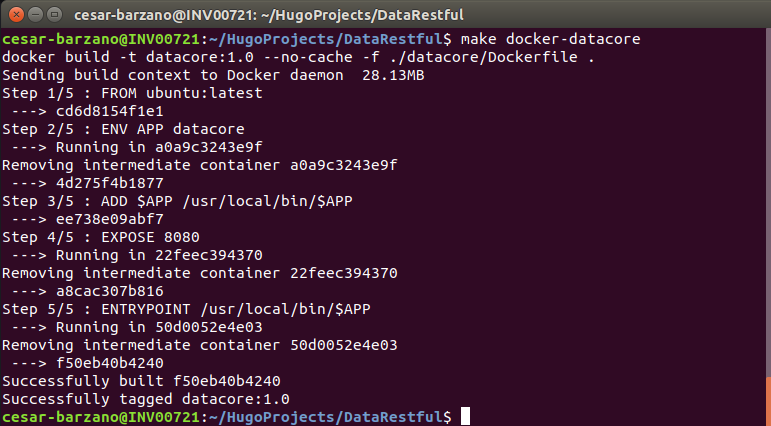
\includegraphics[scale=0.35]{imagenes/make_docker_datacore.png}
\caption{ make docker-datacore }  
\end{figure} 

Puesto que el servicio datacore ha sido implementado con GO, lenguaje compilado capaz de generar ejecutables multiplataforma, la construcción de la imagen es rápida, pues no es necesario instalar nada en ella. En el caso de la imagen docker que representa al servicio de procesamiento python, es necesario instalar las dependencias  necesarias, las cuales son establecidas en el Dockerfile que se muestra a continuación. La imagen que representa este fichero puede ser generada mediante \textbf{make docker-basicpythonprocessor}:

\begin{lstlisting}[language=python,caption={basicPythonProcessor/Dockerfile}]
FROM ubuntu:latest
RUN apt-get update
RUN apt-get install -y python
RUN apt-get install -y python-pip
RUN pip install --upgrade pip



ENV SERVICE_URL http://pythonprocessor:5000/basicOperator
ENV DATARESTFUL_URL http://datacore:8080
ENV APP app.py
ADD . /usr/local/bin/

RUN pip install Flask==0.10.1
RUN pip install requests==2.19.1
RUN pip install urllib3==1.23


EXPOSE 5000
ENTRYPOINT python /usr/local/bin/$APP

\end{lstlisting}

Una vez generadas las imagenes necesarias para los servicios que componen Datarestful podemos levantar la arquitectura completa, para ello se ha definido el siguiente docker-compose.yml


\begin{lstlisting}[language=python,caption={docker-compose.yml}]

version: "2"

services:
  mongodb:
    image: mongo:3.5.6
    ports:
      - 27019:27017

  datacore:
    image: datacore:1.0
    depends_on:
      - mongodb
    ports:
      - "8080:8080"

  pythonprocessor:
    image: basicpythonprocessor:1.0
    depends_on:
      - datacore
    ports:
      - "5000:5000"
\end{lstlisting}


Como se puede observar, para la capa de persistencia se usa una imagen mongoDB oficial, por lo que no es necesaria generarla mediante un Dockerfile, tan solo es necesaria tenerla presente en nuestro sistema o descargarla en caso contrario. Een este fichero se especifica el comportamiento del sistema, es decir, el orden en el que nuestros servicios han de estar disponibles y el orden en el que nuestros servicios han de detenerse.  El servicio que representa la capa de persistencia (mongoDB) será el primero en arrancar, pues el servicio datacore depende de él, siendo este el siguiente en arrancar. El último servicio en arrancar será el procesador python pues depende de datacore para funcionar. Este es el comportamiento nominal, pues datacore necesita mongoDB ya que es el encargado de de interactuar con la base de datos y el resto de procesadores (en este caso solo uno) necesitan a datacore pues la primera acción que realizan estos servicios es el de registrarse como servicio disponible de procesamiento. Cuando uno de estos servicios sufre un fallo y se detiene, se eliminará de la colección de servicios disponibles para el ususario, pues no será capaz de atender peticiones de ninguna clase. Datarestful puede ser levantado mediante \textbf{make datarestful-up}. 

\begin{figure}[H]  
\centering 
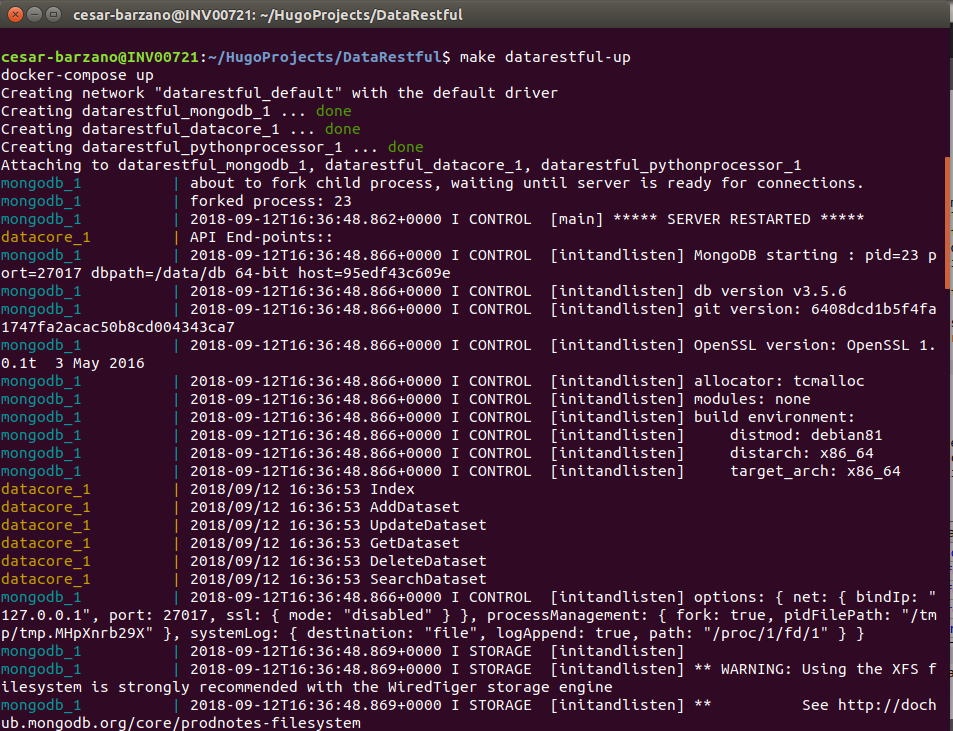
\includegraphics[scale=0.35]{imagenes/make_datarestful_up.png}
\caption{ make datarestful-up }  
\end{figure} 

Se puede apreciar que todos los logs de los servicios que acabamos de levantar se muestran por la misma salida estandar, lo que puede dificultar las tareas debug, para ello, podemos consultar los logs de cada servicio de manera independiente, por ejemplo con make datacore-service-show es posible chequear los logs del servicio datacore o los del servicio de procesamiento:


\begin{figure}[H]  
\centering 
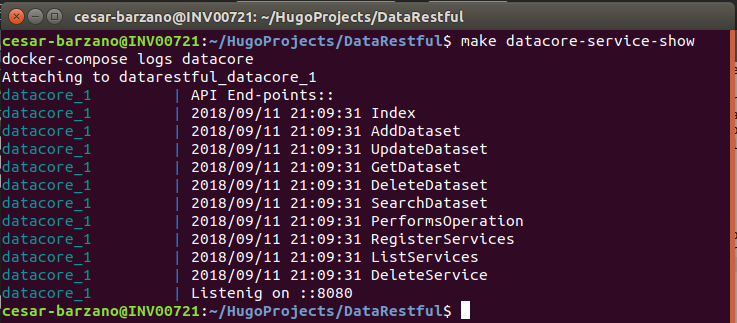
\includegraphics[scale=0.35]{imagenes/datacore-service-show.png}
\caption{ make datacore-service-show }  
\end{figure} 


\begin{figure}[H]  
\centering 
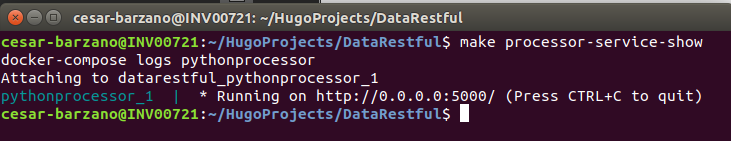
\includegraphics[scale=0.35]{imagenes/processor-service-show.png}
\caption{ make processor-service-show }  
\end{figure} 

Se puede observar que los servicios no han atendido ninguna request, pues solo los hemos arrancado, y la unica petición atendida ha sido por el datacore, realizada por el servicio de procesamiento para darse de alta como servicio disponible. 

Finalmente, cuando se quiera detener Datarestful podemos emplear las reglas down, por ejemplo, podemos detener el sistema completo mediante \textbf{make datarestful-down}  donde se aprecia como los servicios son detenidos en el orden adecuado, primero el procesador basico, seguido del servicio datacore y finalmente la instancia de mongo: 

\begin{figure}[H]  
\centering 
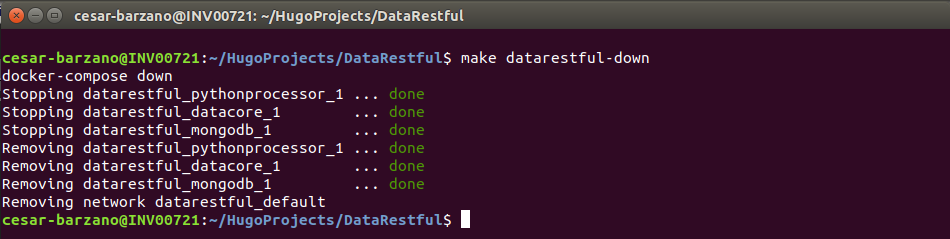
\includegraphics[scale=0.35]{imagenes/datarestful-down.png}
\caption{ make datarestful-down}  
\end{figure} 

 
 
 \section{Caso de Uso}
 
 Con el objetivo de mostrar las funcionalidades implementadas, se va a ejecutar un caso de uso. Al tratarse de una arquitectura basada en servicios REST que carece de frontal, se pueden utilizar herramientas como postman para realizar las distintas peticiones que un usuario de Datarestful realizaría de manera nominal. Teniendo en cuenta herramientas como esta, finalmente se ha decidido implementar el siguiente CLI para interactuar con el sistema mediante el uso del comando curl con funciones de interprete bash: 

\begin{lstlisting}[language=python,caption={resources/cli/datacli.sh}]

#!/usr/bin/env bash
HOST=localhost
PORT=8080

function Datarestful_index() {
  curl -X GET  \
    "http://$HOST:$PORT/" \
    -H 'Content-Type: application/json' \
    -H 'Accept: application/json'
}

function Datarestful_addDataset() {
  TITLE=$1
  DATA=$2
  curl -X POST  \
    "http://$HOST:$PORT/AddDataset" \
    -H 'Content-Type: application/json' \
    -H 'Accept: application/json' \
    -d '{
      "title": "'$TITLE'",
      "data": ["1", "2", "3"]
    }'
}

function Datarestful_getDataset() {
  ID=$1
  curl -X GET  \
    "http://$HOST:$PORT/datasets/$ID" \
    -H 'Content-Type: application/json' \
    -H 'Accept: application/json'
}

function Datarestful_getDatasetByTitle() {
  T=$1
  curl -X GET  \
    "http://$HOST:$PORT/Search/$T" \
    -H 'Content-Type: application/json' \
    -H 'Accept: application/json'
}

function Datarestful_deleteDataset() {
  ID=$1
  curl -X DELETE  \
    "http://$HOST:$PORT/deleteDataset/$ID" \
    -H 'Content-Type: application/json' \
    -H 'Accept: application/json'
}

function Datarestful_updateDataset() {
  ID=$1
  TITLE=$2
  #DATA=[1, 2, 3]
  curl -X PUT  \
    "http://$HOST:$PORT/UpdateDataset" \
    -H 'Content-Type: application/json' \
    -H 'Accept: application/json' \
    -d '{
       "_id": "'$ID'",
      "title": "'$TITLE'",
      "data": ["1111", "2222", "3333"]
    }'
}

function Datarestful_listservices() {
  curl -X GET  \
    "http://$HOST:$PORT/Services/" \
    -H 'Content-Type: application/json' \
    -H 'Accept: application/json'
}

function Datarestful_operation() {
  ID=$1
  VALUE=$2
  OPE=$3
  URL=$4
  curl -X POST  \
    "http://$HOST:$PORT/Operation/" \
    -H 'Content-Type: application/json' \
    -H 'Accept: application/json' \
    -d '{
	    "dataset_id": "'$ID'",
	    "value": "'$VALUE'",
	    "operator": "'$OPE'",
	    "service_url":  "'$URL'"
    }'
}
\end{lstlisting}

Para hablitirar este CLI es necesario abrir una nueva terminal y ejecutar \textbf{source resources/cli/datacli.sh} en la raíz del proyecto, a continuación, si escribimos Data\_ e intentamos tabular para que nos auto-complete la terminal, podemos confirmar que efectivamente las operaciones estan disponibles solo para ser ejecutadas desde esta terminal.  

\begin{figure}[H]  
\centering 
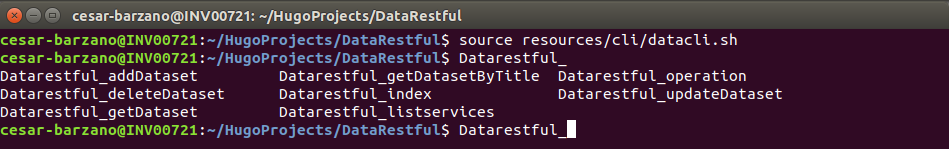
\includegraphics[scale=0.35]{imagenes/cli.png}
\caption{ cli }  
\end{figure} 


Por simplicidad, algunos de los datos que son enviados en el body de las peticiones son estáticos. Para mostrar la usabilidad del sistema y representar un caso de uso, se van a enumerar una serie de pasos o steps con las distintas peticiones que se van a realizar.  

\subsection{Step-1: Servicios Disponibles}

Para comenzar, solo hemos levantado el servicio datacore mediante \textbf{make datacore-service-up}, para que el usuario pueda gestionar los datasets y consultar los servicios de procesamiento disponibles.

El usuario de Datarestful desea conocer los servicios de procesamiento que tiene disponibles, para ello, desde la terminal con el cli cargado, ejecuta \textbf{Datarestful\_listservices} y obtiene una lista vacia, pues aun no hemos levantado el servicio de procesmiento.  

\begin{figure}[H]  
\centering 
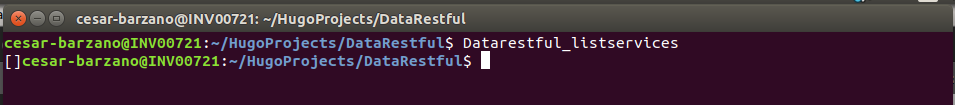
\includegraphics[scale=0.35]{imagenes/list_services.png}
\caption{ Step1- http://\$HOST:\$PORT/Services/ }  
\end{figure} 


Si levantamos el servicio de procesamiento mediante \textbf{make processor-service-up} y el usuario vuelve a ejecutar \textbf{Datarestful\_listservices} desde el cli, esta vez si optiene el servicio que acabamos de levantar, con la información necesaria para futuras operaciones: 

\begin{figure}[H]  
\centering 
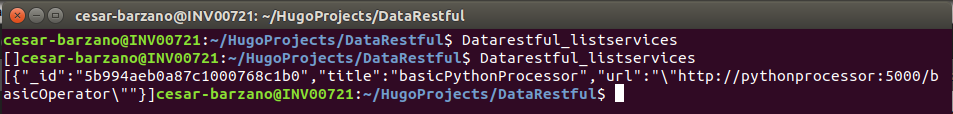
\includegraphics[scale=0.35]{imagenes/list_services2.png}
\caption{ Step 1: http://\$HOST:\$PORT/Services/  }  
\end{figure} 

De manera adicional, podemos chequear los logs del servicio datacore para validar que efectivamente se ha registrado un nuevo servicio de procesamiento. \textbf{NOTA:} Estos logs corresponden a los servicios, un usuario nominal no dispondría de estas trazas. 

\begin{figure}[H]  
\centering 
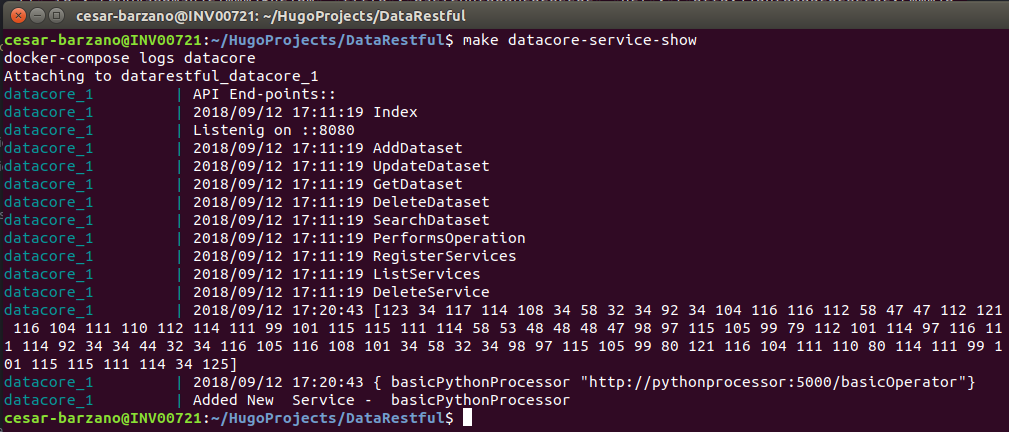
\includegraphics[scale=0.35]{imagenes/add_service.png}
\caption{ make datacore-service-show }  
\end{figure} 

\subsection{Step-2: Gestión de Datasets}

Una vez que el usuario de Dataresful dispone de servicios de procesamiento, lo siguiente que ha de hacer es nutrir al sistema de datos sobre los que realizar procesamiento. Para ello, desde el cli puede obtener todas los datasets de los que dispone ejecutando \textbf{Datarestful\_index}

\begin{figure}[H]  
\centering 
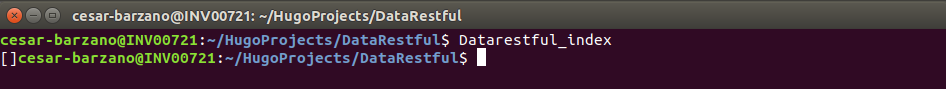
\includegraphics[scale=0.35]{imagenes/index.png}
\caption{ Step 2: http://\$HOST:\$PORT/   }  
\end{figure} 

Puesto que aun no se ha dado de alta ningun dataset, la consulta devuelve una lista vacia. Para dar de alta un dataset generico, desde el cli, el usuario puede ejecutar \textbf{Datarestful\_addDataset step2} enviado una petición POST sobre el end-point \textbf{http://\$HOST:\$PORT/AddDataset} y de nuevo \textbf{Datarestful\_index} devolviendo ahora el dataset estático que se ha definido en el cli: 

\begin{figure}[H]  
\centering 
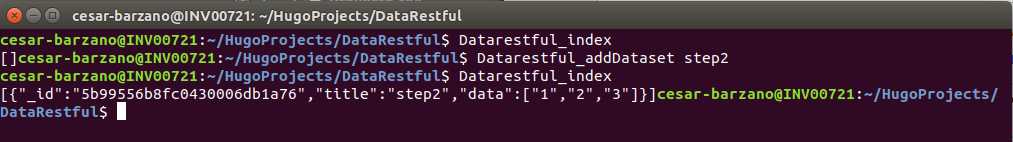
\includegraphics[scale=0.35]{imagenes/add_dataset.png}
\caption{ Step 2: http://\$HOST:\$PORT/   }  
\end{figure} 

El usuario ha realizado varias llamadas a \textbf{Datarestful\_addDataset } con distintos títulos por lo que si consulta todas las datasets mediante \textbf{Datarestful\_index} obtendrá:

\begin{figure}[H]  
\centering 
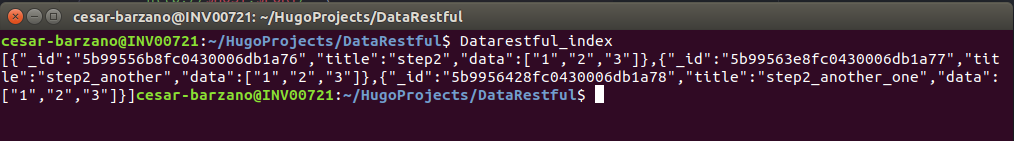
\includegraphics[scale=0.35]{imagenes/many.png}
\caption{ Step 2: http://\$HOST:\$PORT/   }  
\end{figure} 

El usuario puede filtrar los datasets disponibles mediante ID usando \textbf{Datarestful\_getDataset ID}

\begin{figure}[H]  
\centering 
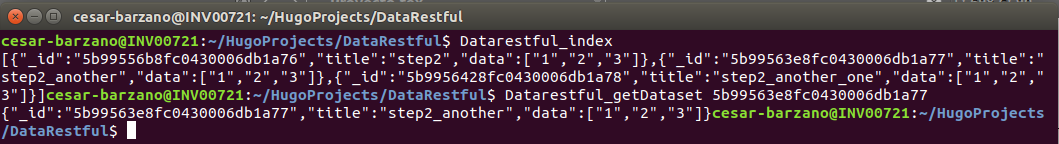
\includegraphics[scale=0.35]{imagenes/id.png}
\caption{ Step 2: http://\$HOST:\$PORT/datasets/\$ID   }  
\end{figure} 

El usuario puede filtrar los datasets disponibles mediante su título usando \textbf{Datarestful\_getDatasetByTitle title}

\begin{figure}[H]  
\centering 
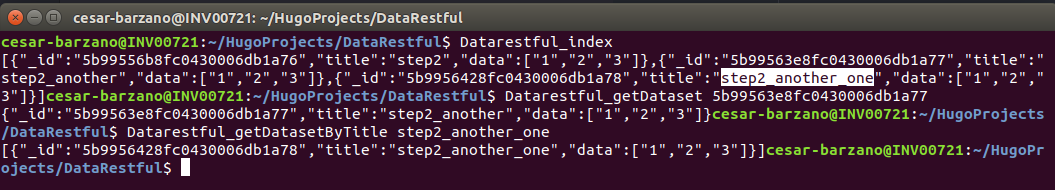
\includegraphics[scale=0.35]{imagenes/string.png}
\caption{ Step 2: http://\$HOST:\$PORT/Search/\$T   }  
\end{figure}

El usuario puede actualizar los datasets disponibles mediante Datarestful\_updateDataset \$ID \$TITLE donde \$ID  corresponde a la \_id del dataset que será actualizado, y \$TITLE al nuevo titulo. En esta operación y por simplificar, los datos con los que se actualizará la dataset en cuestión son estaticos, pero bastaría con componer una PUT request con la siguiente estructura en su body:  

\begin{lstlisting}[language=python,caption={body}]
{
	"_id": "dataset_id_to_update",
    "title": "new_title",
    "data": ["9999", "888", "77","6"]
}

\end{lstlisting}

\begin{figure}[H]  
\centering 
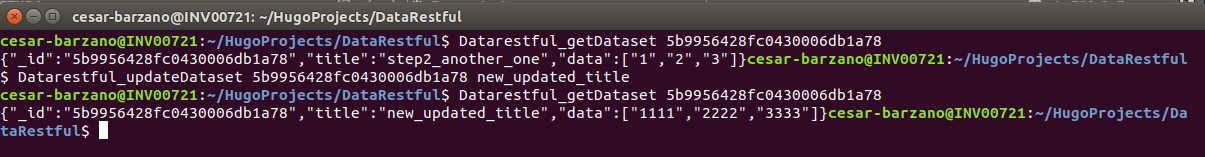
\includegraphics[scale=0.35]{imagenes/update.png}
\caption{ Step 2: http://\$HOST:\$PORT/UpdateDataset }  
\end{figure}


El ususario puede eliminar aquellos datasets que considere oportunos mediante la operación \textbf{Datarestful\_deleteDataset \$ID} donde \$ID corresponde al identificador del dataset en cuestión. 

\begin{figure}[H]  
\centering 
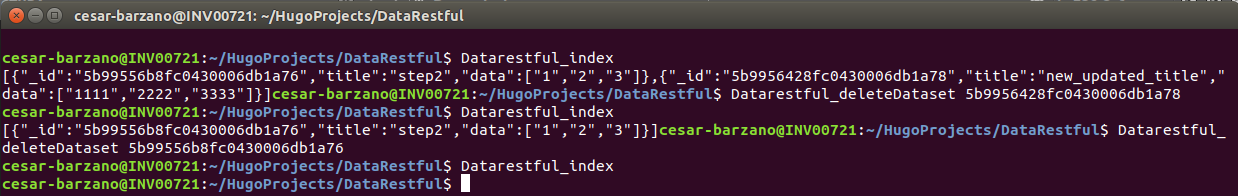
\includegraphics[scale=0.35]{imagenes/delete.png}
\caption{ Step 2: http://\$HOST:\$PORT/deleteDataset/\$ID }  
\end{figure}

\subsection{Step-3: Operaciones}

El siguiente paso es solicitar alguna operación aritmética sobre un dataset, para ello, se puede hacer uso de la función Datarestful\_operation \$ID \$VALUE \$OPE \$URL donde:

\begin{enumerate}
\item \textbf{ID} identificador del dataset a operar 
\item \textbf{VALUE} valor utilizado en la operacion aritmética
\item \textbf{OPE} Operardor representativo de la operación
\item \textbf{URL} dirección del servicio al que delegaremos la operación
\end{enumerate}

Para realizar una operación, el usuario ha de tener algún conjunto de datos declarado en el sistema, debe de haber algun servicio de procesamiento disponible y solicitar una operación, en el siguiente caso, la suma del valor 2 a todo el conjunto de datos:

\begin{figure}[H]  
\centering 
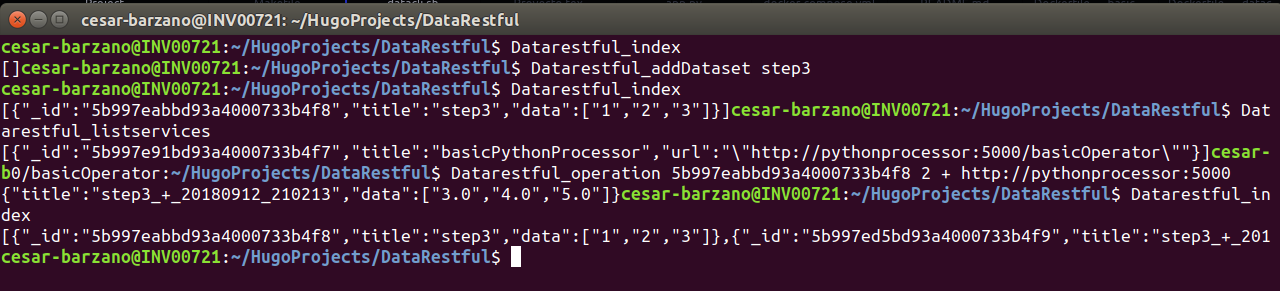
\includegraphics[scale=0.35]{imagenes/ope.png}
\caption{ Step 3: http://\$HOST:\$PORT/Operation/ }  
\end{figure}

El procesador básico soporta multiplicación, resta y división:

\begin{figure}[H]  
\centering 
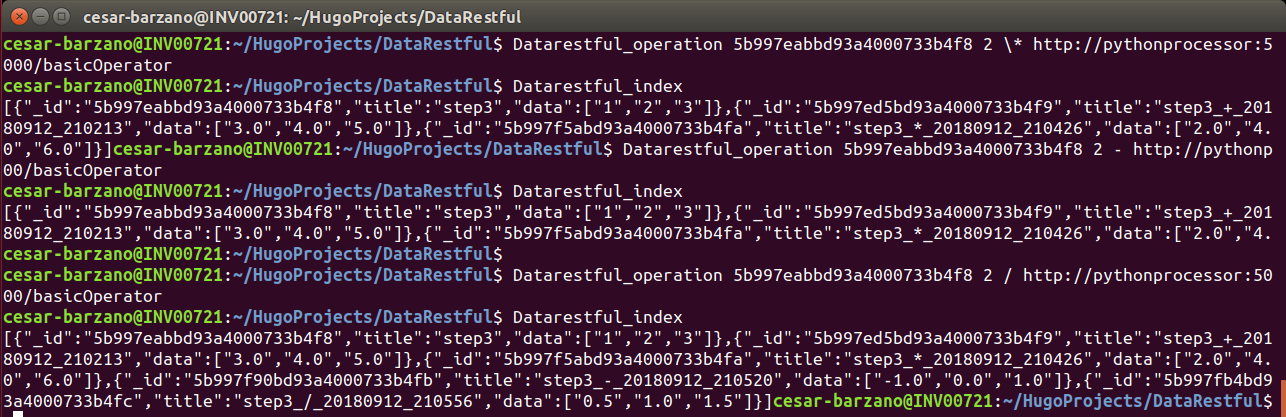
\includegraphics[scale=0.35]{imagenes/ope2.png}
\caption{ Step 3: http://\$HOST:\$PORT/Operation/ }  
\end{figure}

Chequeando los logs del servicio datacore se pueden observar las operaciones solicitadas: 

\begin{figure}[H]  
\centering 
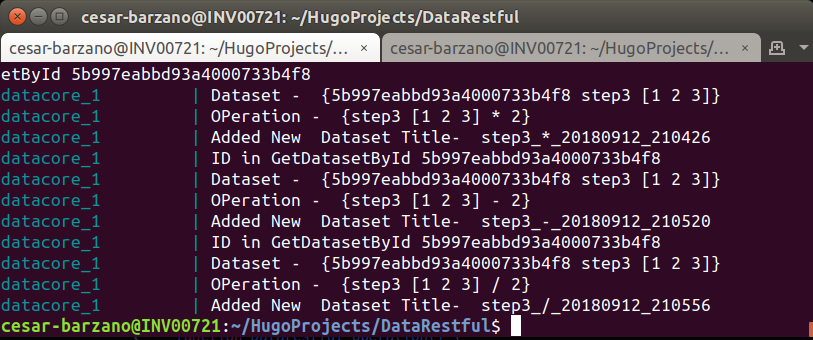
\includegraphics[scale=0.35]{imagenes/ope3.png}
\caption{ Step 3: make datacore-service-show }  
\end{figure}

Chequeando los logs del servicio pythonprocessor se pueden observar las operaciones atendidas: 

\begin{figure}[H]  
\centering 
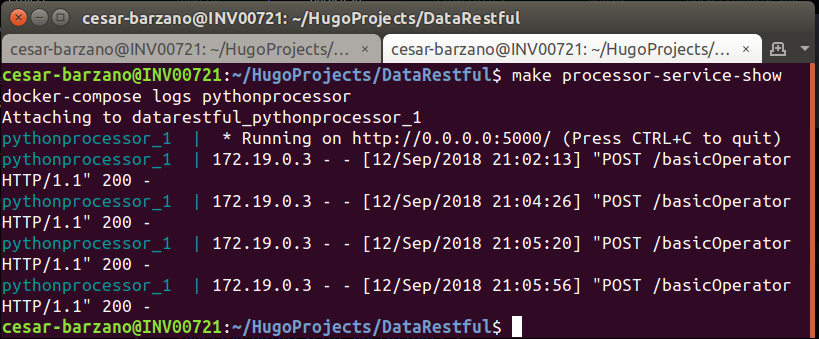
\includegraphics[scale=0.35]{imagenes/ope4.png}
\caption{ Step 3: make processor-service-show }  
\end{figure}


\section{Conclusiones}

El prototipo del sistema resultante cumple con las indicaciones que cliente solicito ya que es facilmente escalable pues soporta tantas operaciones como servicios de procesamiento se registren en el servicio de gestión datacore. La arquitectura orientada a servicios que se ha implementado permite que distintos procesadores, implementados con distintas tecnlogías sean capaces de integrarse como servicio al sistema lo que facilita la actualización de sus capacidades. La base de datos MongoDB esta pensada para grandes cantidades de datos y en el futuro, cuando el rendimiento del sistema se mida en proporciones globales podrá escalarse facilmente mediante una configuración de replica-set donde un conjunto de MongoDBs actuan como una sola. 


El uso de contenedores para la estructuración y pruebas del sistema facilita a los desarrolladores la distribución del sistema ya que no necesitan instalar las dependencias, solo disponer de docker en su sistema, ademas facilita las pruebas y las tareas debug. 
 
 
\chapter{Entrega}

La entrega contiene los siguientes directorios:  

\begin{enumerate}
\item \textbf{basicPythonProcessor} código fuente del servicio de procesamiento.
\item \textbf{datacore:} código fuente del servicio principal de gestión de datos.
\item \textbf{DOC} Ficheros fuente de esta documentación redactada con LaTEX
\item \textbf{resources} Recursos adicionales como el cli.sh
\end{enumerate}

De manera adicional, el directorio raíz contiene este documento en formato PDF a modo de memoria formal, licencia GPL3, herramienta de construcción y especificación de arquitectura. 

 
\begin{thebibliography}{aaaa}

%intro

\bibitem[1]{gogle} \textsc{GOOGLE},
\textit{Google Cloud}
\url{https://cloud.google.com/?hl=es} 



\bibitem[2]{aws} \textsc{AWS},
\textit{Amazon Web Services}
\url{https://aws.amazon.com/es/?nc2=h_lg} 

%Desarrollo

\bibitem[3]{azure} \textsc{azure},
\textit{Microsoft Azure}
\url{https://azure.microsoft.com/es-es/} 


\bibitem[4]{mlab} \textsc{mLAB},
\textit{mLab: Database-as-a-Service for MongoDB}
\url{https://mlab.com/} 

\bibitem[5]{yahoo} \textsc{Yahoo},
\textit{Yahoo}
\url{https://es.yahoo.com/} 

\bibitem[6]{ecs} \textsc{ECS},
\textit{Ether Cloud Services}
\url{http://www.ticbeat.com/innovacion/fintech/inaki-bernal-cto-del-bbva-somos-una-compania-de-software-bastante-mala/} 

\bibitem[7]{api} \textsc{Api Rest},
\textit{Representational State Transfer}
\url{https://bbvaopen4u.com/es/actualidad/api-rest-que-es-y-cuales-son-sus-ventajas-en-el-desarrollo-de-proyectos} 

\bibitem[8]{http} \textsc{HTTP},
\textit{Hypertext Transfer Protocol -- HTTP}
\url{https://www.w3.org/Protocols/rfc2616/rfc2616.html}

\bibitem[9]{py} \textsc{Python},
\textit{Programing Language}
\url{https://www.python.org/}


\bibitem[10]{flask} \textsc{Flask},
\textit{Python Microframework }
\url{http://flask.pocoo.org/}

\bibitem[11]{go} \textsc{GO},
\textit{The Go Programming Language}
\url{https://golang.org/}


\bibitem[12]{mongo} \textsc{MongoDB},
\textit{noSQL Mongo Data Base}
\url{https://www.mongodb.com/}

\bibitem[12]{docker} \textsc{Docker},
\textit{Build, Manage and Secure Your Apps Anywhere. Your Way.}
\url{https://www.docker.com/}


\end{thebibliography}
 


%
%
%%\nocite{*}
%\bibliography{bibliografia/bibliografia}\addcontentsline{toc}{chapter}{Bibliografía}
%\bibliographystyle{miunsrturl}
%
%\appendix

%\input{apendices/manual_usuario/manual_usuario}
%%\input{apendices/paper/paper}
%\input{glosario/entradas_glosario}
% \addcontentsline{toc}{chapter}{Glosario}
% \printglossary

\thispagestyle{empty}

\end{document}
